% Created by tikzDevice version 0.9 on 2015-12-07 11:53:20
% !TEX encoding = UTF-8 Unicode
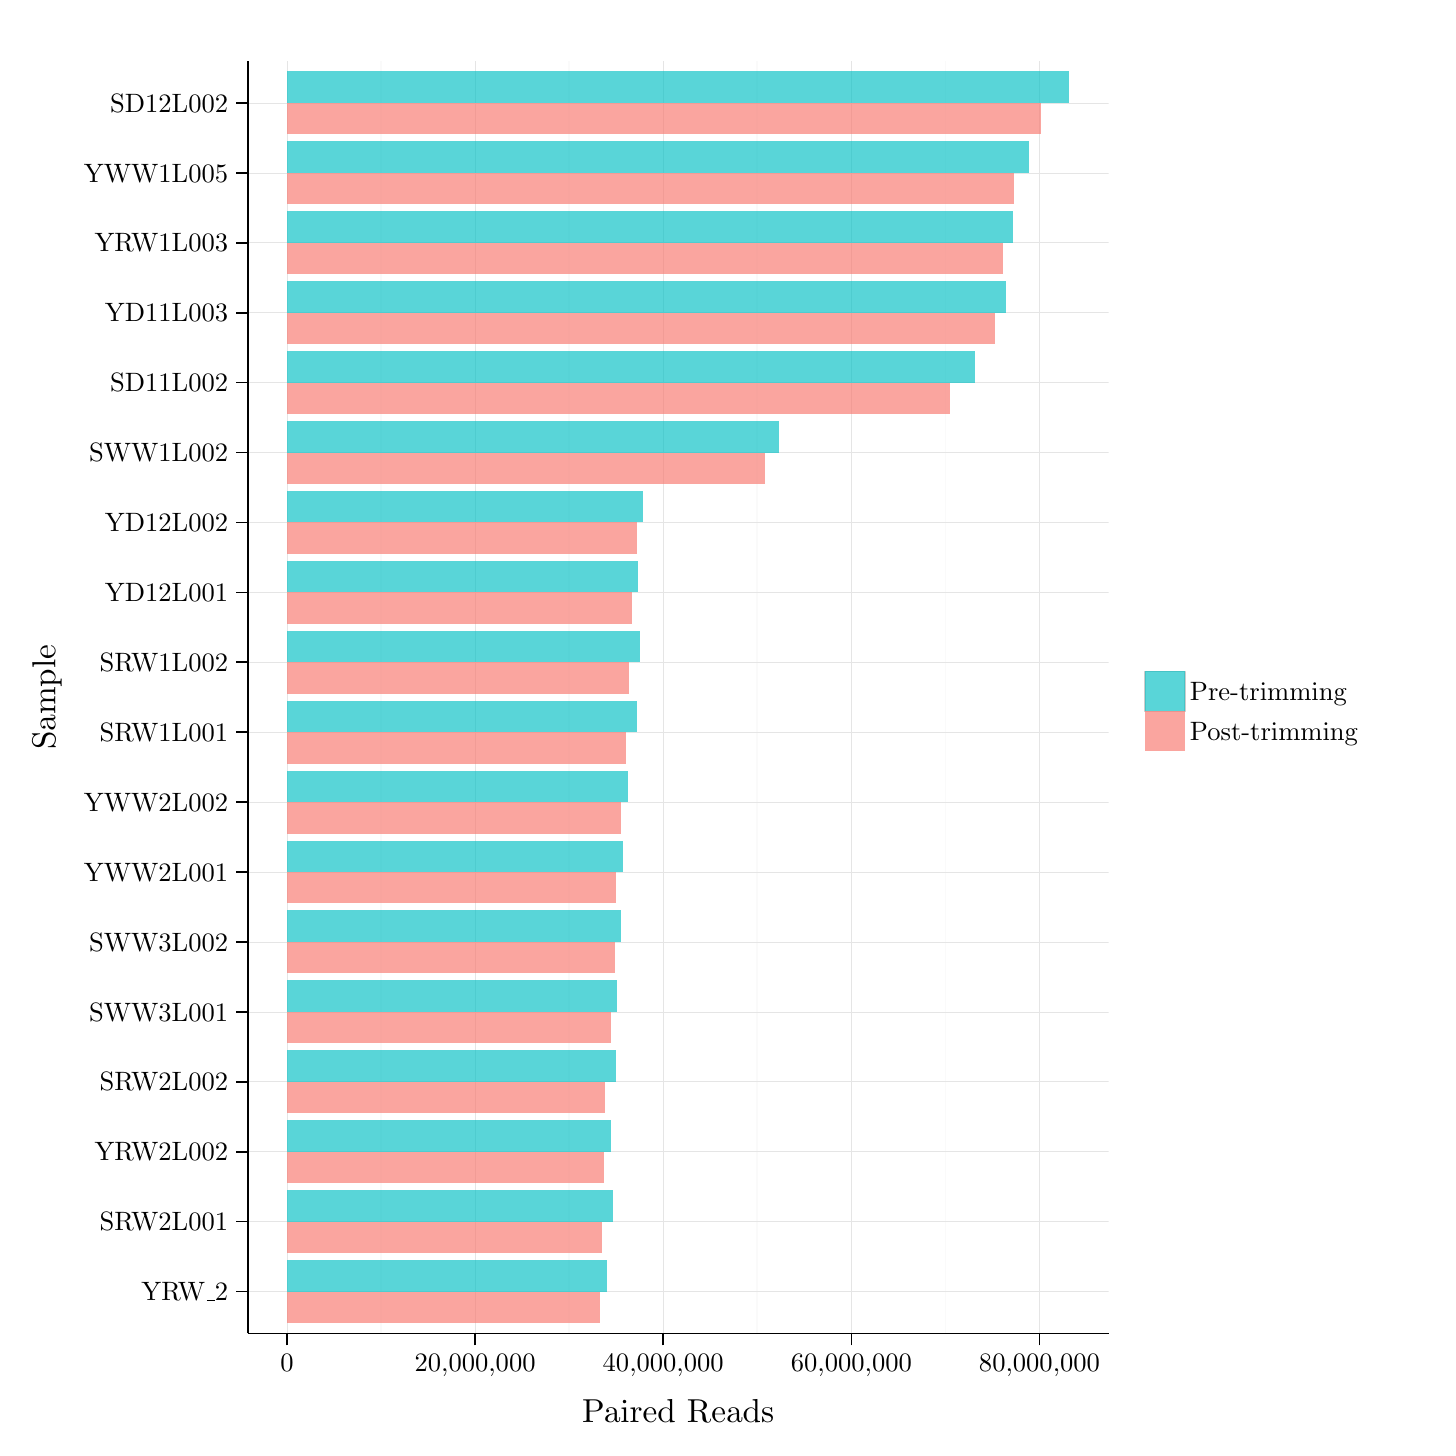
\begin{tikzpicture}[x=1pt,y=1pt]
\definecolor{fillColor}{RGB}{255,255,255}
\path[use as bounding box,fill=fillColor,fill opacity=0.00] (0,0) rectangle (505.89,505.89);
\begin{scope}
\path[clip] (  0.00,  0.00) rectangle (505.89,505.89);
\definecolor{drawColor}{RGB}{255,255,255}
\definecolor{fillColor}{RGB}{255,255,255}

\path[draw=drawColor,line width= 0.6pt,line join=round,line cap=round,fill=fillColor] (  0.00,  0.00) rectangle (505.89,505.89);
\end{scope}
\begin{scope}
\path[clip] ( 79.54, 34.03) rectangle (390.58,493.85);
\definecolor{fillColor}{RGB}{255,255,255}

\path[fill=fillColor] ( 79.54, 34.03) rectangle (390.58,493.85);
\definecolor{drawColor}{gray}{0.98}

\path[draw=drawColor,line width= 0.6pt,line join=round] (127.67, 34.03) --
	(127.67,493.85);

\path[draw=drawColor,line width= 0.6pt,line join=round] (195.66, 34.03) --
	(195.66,493.85);

\path[draw=drawColor,line width= 0.6pt,line join=round] (263.64, 34.03) --
	(263.64,493.85);

\path[draw=drawColor,line width= 0.6pt,line join=round] (331.63, 34.03) --
	(331.63,493.85);
\definecolor{drawColor}{gray}{0.90}

\path[draw=drawColor,line width= 0.2pt,line join=round] ( 79.54, 49.19) --
	(390.58, 49.19);

\path[draw=drawColor,line width= 0.2pt,line join=round] ( 79.54, 74.46) --
	(390.58, 74.46);

\path[draw=drawColor,line width= 0.2pt,line join=round] ( 79.54, 99.72) --
	(390.58, 99.72);

\path[draw=drawColor,line width= 0.2pt,line join=round] ( 79.54,124.99) --
	(390.58,124.99);

\path[draw=drawColor,line width= 0.2pt,line join=round] ( 79.54,150.25) --
	(390.58,150.25);

\path[draw=drawColor,line width= 0.2pt,line join=round] ( 79.54,175.51) --
	(390.58,175.51);

\path[draw=drawColor,line width= 0.2pt,line join=round] ( 79.54,200.78) --
	(390.58,200.78);

\path[draw=drawColor,line width= 0.2pt,line join=round] ( 79.54,226.04) --
	(390.58,226.04);

\path[draw=drawColor,line width= 0.2pt,line join=round] ( 79.54,251.31) --
	(390.58,251.31);

\path[draw=drawColor,line width= 0.2pt,line join=round] ( 79.54,276.57) --
	(390.58,276.57);

\path[draw=drawColor,line width= 0.2pt,line join=round] ( 79.54,301.84) --
	(390.58,301.84);

\path[draw=drawColor,line width= 0.2pt,line join=round] ( 79.54,327.10) --
	(390.58,327.10);

\path[draw=drawColor,line width= 0.2pt,line join=round] ( 79.54,352.36) --
	(390.58,352.36);

\path[draw=drawColor,line width= 0.2pt,line join=round] ( 79.54,377.63) --
	(390.58,377.63);

\path[draw=drawColor,line width= 0.2pt,line join=round] ( 79.54,402.89) --
	(390.58,402.89);

\path[draw=drawColor,line width= 0.2pt,line join=round] ( 79.54,428.16) --
	(390.58,428.16);

\path[draw=drawColor,line width= 0.2pt,line join=round] ( 79.54,453.42) --
	(390.58,453.42);

\path[draw=drawColor,line width= 0.2pt,line join=round] ( 79.54,478.69) --
	(390.58,478.69);

\path[draw=drawColor,line width= 0.2pt,line join=round] ( 93.68, 34.03) --
	( 93.68,493.85);

\path[draw=drawColor,line width= 0.2pt,line join=round] (161.67, 34.03) --
	(161.67,493.85);

\path[draw=drawColor,line width= 0.2pt,line join=round] (229.65, 34.03) --
	(229.65,493.85);

\path[draw=drawColor,line width= 0.2pt,line join=round] (297.63, 34.03) --
	(297.63,493.85);

\path[draw=drawColor,line width= 0.2pt,line join=round] (365.62, 34.03) --
	(365.62,493.85);
\definecolor{fillColor}{RGB}{0,191,196}

\path[fill=fillColor,fill opacity=0.65] ( 93.68, 49.19) rectangle (209.37, 60.56);
\definecolor{fillColor}{RGB}{248,118,109}

\path[fill=fillColor,fill opacity=0.65] ( 93.68, 37.82) rectangle (206.96, 49.19);
\definecolor{fillColor}{RGB}{0,191,196}

\path[fill=fillColor,fill opacity=0.65] ( 93.68, 74.46) rectangle (211.57, 85.83);
\definecolor{fillColor}{RGB}{248,118,109}

\path[fill=fillColor,fill opacity=0.65] ( 93.68, 63.09) rectangle (207.68, 74.46);
\definecolor{fillColor}{RGB}{0,191,196}

\path[fill=fillColor,fill opacity=0.65] ( 93.68, 99.72) rectangle (210.90,111.09);
\definecolor{fillColor}{RGB}{248,118,109}

\path[fill=fillColor,fill opacity=0.65] ( 93.68, 88.35) rectangle (208.43, 99.72);
\definecolor{fillColor}{RGB}{0,191,196}

\path[fill=fillColor,fill opacity=0.65] ( 93.68,124.99) rectangle (212.72,136.36);
\definecolor{fillColor}{RGB}{248,118,109}

\path[fill=fillColor,fill opacity=0.65] ( 93.68,113.62) rectangle (208.71,124.99);
\definecolor{fillColor}{RGB}{0,191,196}

\path[fill=fillColor,fill opacity=0.65] ( 93.68,150.25) rectangle (212.78,161.62);
\definecolor{fillColor}{RGB}{248,118,109}

\path[fill=fillColor,fill opacity=0.65] ( 93.68,138.88) rectangle (210.64,150.25);
\definecolor{fillColor}{RGB}{0,191,196}

\path[fill=fillColor,fill opacity=0.65] ( 93.68,175.51) rectangle (214.43,186.88);
\definecolor{fillColor}{RGB}{248,118,109}

\path[fill=fillColor,fill opacity=0.65] ( 93.68,164.15) rectangle (212.23,175.51);
\definecolor{fillColor}{RGB}{0,191,196}

\path[fill=fillColor,fill opacity=0.65] ( 93.68,200.78) rectangle (215.15,212.15);
\definecolor{fillColor}{RGB}{248,118,109}

\path[fill=fillColor,fill opacity=0.65] ( 93.68,189.41) rectangle (212.75,200.78);
\definecolor{fillColor}{RGB}{0,191,196}

\path[fill=fillColor,fill opacity=0.65] ( 93.68,226.04) rectangle (216.85,237.41);
\definecolor{fillColor}{RGB}{248,118,109}

\path[fill=fillColor,fill opacity=0.65] ( 93.68,214.67) rectangle (214.37,226.04);
\definecolor{fillColor}{RGB}{0,191,196}

\path[fill=fillColor,fill opacity=0.65] ( 93.68,251.31) rectangle (220.19,262.68);
\definecolor{fillColor}{RGB}{248,118,109}

\path[fill=fillColor,fill opacity=0.65] ( 93.68,239.94) rectangle (216.27,251.31);
\definecolor{fillColor}{RGB}{0,191,196}

\path[fill=fillColor,fill opacity=0.65] ( 93.68,276.57) rectangle (221.27,287.94);
\definecolor{fillColor}{RGB}{248,118,109}

\path[fill=fillColor,fill opacity=0.65] ( 93.68,265.20) rectangle (217.26,276.57);
\definecolor{fillColor}{RGB}{0,191,196}

\path[fill=fillColor,fill opacity=0.65] ( 93.68,301.84) rectangle (220.66,313.21);
\definecolor{fillColor}{RGB}{248,118,109}

\path[fill=fillColor,fill opacity=0.65] ( 93.68,290.47) rectangle (218.54,301.84);
\definecolor{fillColor}{RGB}{0,191,196}

\path[fill=fillColor,fill opacity=0.65] ( 93.68,327.10) rectangle (222.42,338.47);
\definecolor{fillColor}{RGB}{248,118,109}

\path[fill=fillColor,fill opacity=0.65] ( 93.68,315.73) rectangle (220.23,327.10);
\definecolor{fillColor}{RGB}{0,191,196}

\path[fill=fillColor,fill opacity=0.65] ( 93.68,352.36) rectangle (271.60,363.73);
\definecolor{fillColor}{RGB}{248,118,109}

\path[fill=fillColor,fill opacity=0.65] ( 93.68,341.00) rectangle (266.36,352.36);
\definecolor{fillColor}{RGB}{0,191,196}

\path[fill=fillColor,fill opacity=0.65] ( 93.68,377.63) rectangle (342.29,389.00);
\definecolor{fillColor}{RGB}{248,118,109}

\path[fill=fillColor,fill opacity=0.65] ( 93.68,366.26) rectangle (333.38,377.63);
\definecolor{fillColor}{RGB}{0,191,196}

\path[fill=fillColor,fill opacity=0.65] ( 93.68,402.89) rectangle (353.40,414.26);
\definecolor{fillColor}{RGB}{248,118,109}

\path[fill=fillColor,fill opacity=0.65] ( 93.68,391.52) rectangle (349.70,402.89);
\definecolor{fillColor}{RGB}{0,191,196}

\path[fill=fillColor,fill opacity=0.65] ( 93.68,428.16) rectangle (356.00,439.53);
\definecolor{fillColor}{RGB}{248,118,109}

\path[fill=fillColor,fill opacity=0.65] ( 93.68,416.79) rectangle (352.39,428.16);
\definecolor{fillColor}{RGB}{0,191,196}

\path[fill=fillColor,fill opacity=0.65] ( 93.68,453.42) rectangle (361.79,464.79);
\definecolor{fillColor}{RGB}{248,118,109}

\path[fill=fillColor,fill opacity=0.65] ( 93.68,442.05) rectangle (356.31,453.42);
\definecolor{fillColor}{RGB}{0,191,196}

\path[fill=fillColor,fill opacity=0.65] ( 93.68,478.69) rectangle (376.44,490.06);
\definecolor{fillColor}{RGB}{248,118,109}

\path[fill=fillColor,fill opacity=0.65] ( 93.68,467.32) rectangle (366.03,478.69);
\end{scope}
\begin{scope}
\path[clip] (  0.00,  0.00) rectangle (505.89,505.89);
\definecolor{drawColor}{RGB}{0,0,0}

\path[draw=drawColor,line width= 0.6pt,line join=round] ( 79.54, 34.03) --
	( 79.54,493.85);
\end{scope}
\begin{scope}
\path[clip] (  0.00,  0.00) rectangle (505.89,505.89);
\definecolor{drawColor}{RGB}{0,0,0}

\node[text=drawColor,anchor=base east,inner sep=0pt, outer sep=0pt, scale=  0.96] at ( 72.43, 45.89) {YRW\_2};

\node[text=drawColor,anchor=base east,inner sep=0pt, outer sep=0pt, scale=  0.96] at ( 72.43, 71.15) {SRW2L001};

\node[text=drawColor,anchor=base east,inner sep=0pt, outer sep=0pt, scale=  0.96] at ( 72.43, 96.42) {YRW2L002};

\node[text=drawColor,anchor=base east,inner sep=0pt, outer sep=0pt, scale=  0.96] at ( 72.43,121.68) {SRW2L002};

\node[text=drawColor,anchor=base east,inner sep=0pt, outer sep=0pt, scale=  0.96] at ( 72.43,146.94) {SWW3L001};

\node[text=drawColor,anchor=base east,inner sep=0pt, outer sep=0pt, scale=  0.96] at ( 72.43,172.21) {SWW3L002};

\node[text=drawColor,anchor=base east,inner sep=0pt, outer sep=0pt, scale=  0.96] at ( 72.43,197.47) {YWW2L001};

\node[text=drawColor,anchor=base east,inner sep=0pt, outer sep=0pt, scale=  0.96] at ( 72.43,222.74) {YWW2L002};

\node[text=drawColor,anchor=base east,inner sep=0pt, outer sep=0pt, scale=  0.96] at ( 72.43,248.00) {SRW1L001};

\node[text=drawColor,anchor=base east,inner sep=0pt, outer sep=0pt, scale=  0.96] at ( 72.43,273.27) {SRW1L002};

\node[text=drawColor,anchor=base east,inner sep=0pt, outer sep=0pt, scale=  0.96] at ( 72.43,298.53) {YD12L001};

\node[text=drawColor,anchor=base east,inner sep=0pt, outer sep=0pt, scale=  0.96] at ( 72.43,323.79) {YD12L002};

\node[text=drawColor,anchor=base east,inner sep=0pt, outer sep=0pt, scale=  0.96] at ( 72.43,349.06) {SWW1L002};

\node[text=drawColor,anchor=base east,inner sep=0pt, outer sep=0pt, scale=  0.96] at ( 72.43,374.32) {SD11L002};

\node[text=drawColor,anchor=base east,inner sep=0pt, outer sep=0pt, scale=  0.96] at ( 72.43,399.59) {YD11L003};

\node[text=drawColor,anchor=base east,inner sep=0pt, outer sep=0pt, scale=  0.96] at ( 72.43,424.85) {YRW1L003};

\node[text=drawColor,anchor=base east,inner sep=0pt, outer sep=0pt, scale=  0.96] at ( 72.43,450.12) {YWW1L005};

\node[text=drawColor,anchor=base east,inner sep=0pt, outer sep=0pt, scale=  0.96] at ( 72.43,475.38) {SD12L002};
\end{scope}
\begin{scope}
\path[clip] (  0.00,  0.00) rectangle (505.89,505.89);
\definecolor{drawColor}{RGB}{0,0,0}

\path[draw=drawColor,line width= 0.6pt,line join=round] ( 75.28, 49.19) --
	( 79.54, 49.19);

\path[draw=drawColor,line width= 0.6pt,line join=round] ( 75.28, 74.46) --
	( 79.54, 74.46);

\path[draw=drawColor,line width= 0.6pt,line join=round] ( 75.28, 99.72) --
	( 79.54, 99.72);

\path[draw=drawColor,line width= 0.6pt,line join=round] ( 75.28,124.99) --
	( 79.54,124.99);

\path[draw=drawColor,line width= 0.6pt,line join=round] ( 75.28,150.25) --
	( 79.54,150.25);

\path[draw=drawColor,line width= 0.6pt,line join=round] ( 75.28,175.51) --
	( 79.54,175.51);

\path[draw=drawColor,line width= 0.6pt,line join=round] ( 75.28,200.78) --
	( 79.54,200.78);

\path[draw=drawColor,line width= 0.6pt,line join=round] ( 75.28,226.04) --
	( 79.54,226.04);

\path[draw=drawColor,line width= 0.6pt,line join=round] ( 75.28,251.31) --
	( 79.54,251.31);

\path[draw=drawColor,line width= 0.6pt,line join=round] ( 75.28,276.57) --
	( 79.54,276.57);

\path[draw=drawColor,line width= 0.6pt,line join=round] ( 75.28,301.84) --
	( 79.54,301.84);

\path[draw=drawColor,line width= 0.6pt,line join=round] ( 75.28,327.10) --
	( 79.54,327.10);

\path[draw=drawColor,line width= 0.6pt,line join=round] ( 75.28,352.36) --
	( 79.54,352.36);

\path[draw=drawColor,line width= 0.6pt,line join=round] ( 75.28,377.63) --
	( 79.54,377.63);

\path[draw=drawColor,line width= 0.6pt,line join=round] ( 75.28,402.89) --
	( 79.54,402.89);

\path[draw=drawColor,line width= 0.6pt,line join=round] ( 75.28,428.16) --
	( 79.54,428.16);

\path[draw=drawColor,line width= 0.6pt,line join=round] ( 75.28,453.42) --
	( 79.54,453.42);

\path[draw=drawColor,line width= 0.6pt,line join=round] ( 75.28,478.69) --
	( 79.54,478.69);
\end{scope}
\begin{scope}
\path[clip] (  0.00,  0.00) rectangle (505.89,505.89);
\definecolor{drawColor}{RGB}{0,0,0}

\path[draw=drawColor,line width= 0.6pt,line join=round] ( 79.54, 34.03) --
	(390.58, 34.03);
\end{scope}
\begin{scope}
\path[clip] (  0.00,  0.00) rectangle (505.89,505.89);
\definecolor{drawColor}{RGB}{0,0,0}

\path[draw=drawColor,line width= 0.6pt,line join=round] ( 93.68, 29.77) --
	( 93.68, 34.03);

\path[draw=drawColor,line width= 0.6pt,line join=round] (161.67, 29.77) --
	(161.67, 34.03);

\path[draw=drawColor,line width= 0.6pt,line join=round] (229.65, 29.77) --
	(229.65, 34.03);

\path[draw=drawColor,line width= 0.6pt,line join=round] (297.63, 29.77) --
	(297.63, 34.03);

\path[draw=drawColor,line width= 0.6pt,line join=round] (365.62, 29.77) --
	(365.62, 34.03);
\end{scope}
\begin{scope}
\path[clip] (  0.00,  0.00) rectangle (505.89,505.89);
\definecolor{drawColor}{RGB}{0,0,0}

\node[text=drawColor,anchor=base,inner sep=0pt, outer sep=0pt, scale=  0.96] at ( 93.68, 20.31) {0};

\node[text=drawColor,anchor=base,inner sep=0pt, outer sep=0pt, scale=  0.96] at (161.67, 20.31) {20,000,000};

\node[text=drawColor,anchor=base,inner sep=0pt, outer sep=0pt, scale=  0.96] at (229.65, 20.31) {40,000,000};

\node[text=drawColor,anchor=base,inner sep=0pt, outer sep=0pt, scale=  0.96] at (297.63, 20.31) {60,000,000};

\node[text=drawColor,anchor=base,inner sep=0pt, outer sep=0pt, scale=  0.96] at (365.62, 20.31) {80,000,000};
\end{scope}
\begin{scope}
\path[clip] (  0.00,  0.00) rectangle (505.89,505.89);
\definecolor{drawColor}{RGB}{0,0,0}

\node[text=drawColor,anchor=base,inner sep=0pt, outer sep=0pt, scale=  1.20] at (235.06,  2) {Paired Reads};
\end{scope}
\begin{scope}
\path[clip] (  0.00,  0.00) rectangle (505.89,505.89);
\definecolor{drawColor}{RGB}{0,0,0}

\node[text=drawColor,rotate= 90.00,anchor=base,inner sep=0pt, outer sep=0pt, scale=  1.20] at ( 10,263.94) {Sample};
\end{scope}
\begin{scope}
\path[clip] (  0.00,  0.00) rectangle (505.89,505.89);
\definecolor{fillColor}{RGB}{255,255,255}

\path[fill=fillColor] (399.45,240.10) rectangle (484.98,287.78);
\end{scope}
\begin{scope}
\path[clip] (  0.00,  0.00) rectangle (505.89,505.89);
\definecolor{drawColor}{gray}{0.80}
\definecolor{fillColor}{RGB}{255,255,255}

\path[draw=drawColor,line width= 0.6pt,line join=round,line cap=round,fill=fillColor] (403.72,258.82) rectangle (418.17,273.27);
\end{scope}
\begin{scope}
\path[clip] (  0.00,  0.00) rectangle (505.89,505.89);
\definecolor{fillColor}{RGB}{248,118,109}

\path[fill=fillColor,fill opacity=0.65] (403.72,244.37) rectangle (418.17,258.82);

\path[] (403.72,258.82) --
	(418.17,273.27);
\end{scope}
\begin{scope}
\path[clip] (  0.00,  0.00) rectangle (505.89,505.89);
\definecolor{drawColor}{gray}{0.80}
\definecolor{fillColor}{RGB}{255,255,255}

%\path[draw=drawColor,line width= 0.6pt,line join=round,line cap=round,fill=fillColor] (403.72,244.37) rectangle (418.17,258.82);
\end{scope}
\begin{scope}
\path[clip] (  0.00,  0.00) rectangle (505.89,505.89);
\definecolor{fillColor}{RGB}{0,191,196}

\path[fill=fillColor,fill opacity=0.65] (403.72,258.82) rectangle (418.17,273.27);

\path[] (403.72,244.37) --
	(418.17,258.82);
\end{scope}
\begin{scope}
\path[clip] (  0.00,  0.00) rectangle (505.89,505.89);
\definecolor{drawColor}{RGB}{0,0,0}

\node[text=drawColor,anchor=base west,inner sep=0pt, outer sep=0pt, scale=  0.96] at (419.98,262.74) {Pre-trimming};
\end{scope}
\begin{scope}
\path[clip] (  0.00,  0.00) rectangle (505.89,505.89);
\definecolor{drawColor}{RGB}{0,0,0}

\node[text=drawColor,anchor=base west,inner sep=0pt, outer sep=0pt, scale=  0.96] at (419.98,248.29) {Post-trimming};
\end{scope}
\end{tikzpicture}
